\documentclass[a4paper,12pt]{article}
\usepackage[margin=2.5cm]{geometry}
\usepackage{authblk}
\usepackage{amsmath,amssymb,graphicx,hyperref,bm,bbm}
\usepackage{booktabs}
\usepackage{microtype}
\usepackage{tikz}
% Two-column overflow prevention
\tolerance=1500
\emergencystretch=1.5em
\usetikzlibrary{decorations.pathmorphing,arrows.meta,calc}
% ESFT core symbols
% Qoppa (Ϙ): uppercase archaic Greek, pronounced "QOPPA" (not "koppa")
% Unicode U+03D8 = Ϙ (uppercase), U+03D9 = ϙ (lowercase)
% For XeLaTeX/LuaLaTeX: \newcommand{\Qoppa}{\text{Ϙ}}
\newcommand{\Qoppa}{\mathcal{Q}} % Uppercase Qoppa (pdfLaTeX fallback)
\newcommand{\qoppa}{\Qoppa} % backward compat alias
\newcommand{\Phifield}{\Phi} % Energy string field: Φ ≡ ∇Θ
\newcommand{\fsol}{f_{\rm s}}

\newcommand{\vev}[1]{\langle #1 \rangle}
\newcommand{\abs}[1]{|#1|}
\newcommand{\order}[1]{\mathcal{O}(#1)}
\newcommand{\tr}{\mathrm{Tr}}

\begin{document}

\title{Emergent gauge symmetry from Hopf soliton topology in ESFT}

\author{Jesse C.P. Won Ting}
\affil{Independent Researcher}

\begin{abstract}We derive both non-Abelian gauge groups of the Standard Model---SU(2)
weak isospin and SU(3) color---from the symmetries of topological
solitons in the compact phase field $\Theta \in [0,2\pi)$ introduced
in Paper~I.

For SU(2): a single hedgehog soliton with odd topological charge $n$
possesses three rotational zero modes. The Finkelstein--Rubinstein
theorem forces their quantization onto SU(2) (not SO(3))
representations, with the ground state an isospin-1/2 doublet.
The Berry connection of these zero modes is an SU(2) gauge field,
exponentially localized within the soliton core ($r \lesssim a$),
yielding an effective range consistent with the weak scale
$\Lambda_{\mathrm{core}} = \hbar c/a \approx 73$~GeV.

For SU(3): the rank-3 soliton sector of Paper~I decomposes into
three identical Hopf solitons whose permutation symmetry $S_3$ is
identical to the Weyl group $W(A_2)$ of SU(3). This mathematical
identity yields: (i)~Casimir scaling of string tensions for six
representations, matching lattice QCD to $<\!3\%$ with zero free
parameters; (ii)~a complete glueball $J^{PC}$ mass spectrum with
four independent predictions at $\sim\!4\%$ RMS accuracy; and
(iii)~rigid-rotor scaling $M \propto J(J+1)$ confirmed over
Regge-string scaling $M^2 \propto J$.

The residual U(1) of the outer phase field provides electromagnetism.
We show that Adams' theorem on Hopf fibrations, combined with the
non-associativity of the octonions, topologically forbids a fourth
gauge interaction: the Standard Model gauge group
$\mathrm{SU}(3) \times \mathrm{SU}(2) \times \mathrm{U}(1)$ is
the unique structure compatible with the division-algebra
classification of Hopf maps.
\end{abstract}

\maketitle

\noindent\textbf{Keywords:} topological soliton, gauge group emergence, SU(3), SU(2), Casimir scaling, glueball spectrum, Weyl group, Hopf fibration, Adams theorem


%======================================================================
\section{Introduction}
\label{sec:intro}
%======================================================================

The Standard Model of particle physics rests on the gauge group
$\mathrm{SU}(3) \times \mathrm{SU}(2) \times \mathrm{U}(1)$.
This structure is among the most precisely tested in all of science,
yet its \emph{origin} remains unexplained: the gauge group is an
input axiom, not a derived consequence. Why three non-Abelian
factors? Why these particular groups? Why not SU(5), SO(10), or
$E_8$?

Grand unified theories embed the Standard Model group into a larger
simple group, but this merely defers the question: why that particular
embedding? String theory compactifications can produce
$\mathrm{SU}(3) \times \mathrm{SU}(2) \times \mathrm{U}(1)$, but
the landscape of $\sim\!10^{500}$ vacua offers no unique selection.
What is lacking is a \emph{derivation} from a smaller set of
principles.

In Paper~I~\cite{PaperI} we showed that a compact phase field
$\Theta \in [0,2\pi)$, subject only to topological quantization and
energy finiteness, produces a single coherence scale $a$ that
generates falsifiable predictions across seven physical domains.
In this paper we show that the \emph{same} field, with no additional
structure, produces the full non-Abelian gauge content of the
Standard Model.

The argument proceeds in four steps:
\begin{enumerate}
 \item A single soliton's rotational zero modes, quantized via the
 Finkelstein--Rubinstein theorem~\cite{FR1968}, yield
 \textbf{SU(2)} weak isospin (§\ref{sec:su2}).
 \item Three identical solitons in the rank-3 sector, whose
 permutation symmetry $S_3 = W(A_2)$ is the Weyl group of SU(3),
 yield \textbf{SU(3)} color (§\ref{sec:su3}), with quantitative
 verification via Casimir scaling (§\ref{sec:casimir}) and the
 glueball spectrum (§\ref{sec:glueball}).
 \item The outer $S^1$ phase field provides \textbf{U(1)}
 electromagnetism (§\ref{sec:u1}).
 \item Adams' theorem~\cite{Adams1960} on Hopf fibrations forbids
 further gauge groups: there is no fourth force (§\ref{sec:adams}).
\end{enumerate}

Each step rests on established mathematical theorems applied to the
soliton structure of Paper~I\@. No new fields, parameters, or
assumptions are introduced. The only input is $\Theta \in S^1$
with finite energy.


%======================================================================
\section{Framework and notation}
\label{sec:framework}
%======================================================================

We briefly restate the ESFT foundations established in
Paper~I~\cite{PaperI} and fix notation for the present work.

\subsection{The phase field and its gradient}

The sole ontological primitive is a compact scalar field
\begin{equation}
\label{eq:theta}
 \Theta: \mathbb{R}^{3,1} \to S^1, \qquad \Theta \sim \Theta + 2\pi.
\end{equation}
The \emph{energy string field} is its spatial gradient:
\begin{equation}
\label{eq:phi}
 \boxed{\varphi \equiv \nabla\Theta.}
\end{equation}
All physical observables in ESFT are constructed from $\varphi$ and
its derivatives. The compactness of $\Theta$ enforces topological
quantization: for any closed loop $\gamma$ encircling a defect,
\begin{equation}
\label{eq:winding}
 \oint_\gamma \varphi \cdot d\boldsymbol{\ell} = 2\pi n,
 \quad n \in \mathbb{Z}.
\end{equation}

\subsection{Soliton structure and the coherence scale}

A topological soliton is a field configuration with $n \neq 0$,
stabilized by the winding number. Energy finiteness forces a
\emph{two-range profile}:
\begin{equation}
\label{eq:tworange}
 |\varphi(r)| \sim
 \begin{cases}
 n/a & r \lesssim a, \\
 n/r & r \gg a,
 \end{cases}
\end{equation}
where $a$ is the \emph{coherence scale} (core radius).
The dedicated symbol $\qoppa$ (Qoppa, archaic Greek), introduced in
Paper~I as the canonical notation for the ESFT coherence scale, is
defined by:
\begin{equation}
\label{eq:qoppa}
 \qoppa \;\equiv\; a \;\equiv\; \text{coherence scale of the soliton core}.
\end{equation}
In this paper we use $a$ and $\qoppa$ interchangeably; in Paper~III,
$\qoppa$ serves as the primary symbol.

Paper~I constrained $\qoppa$ from precision atomic spectroscopy:
\begin{equation}
\label{eq:avalue}
 \qoppa = (2.701 \pm 0.003) \times 10^{-3}\;\mathrm{fm},
\end{equation}
with core energy scale
\begin{equation}
\label{eq:avalue2}
 \Lambda_{\mathrm{core}} \equiv \frac{\hbar c}{\qoppa}
 = 73.1\;\mathrm{GeV}.
\end{equation}

\subsection{Four-dimensional extension}

The covariant generalization of $\varphi$ is the four-gradient:
\begin{equation}
\label{eq:4grad}
 \Phi_\mu \equiv \partial_\mu \Theta
 = \left(\frac{1}{c}\partial_t\Theta,\;\nabla\Theta\right)
 = \left(\frac{1}{c}\partial_t\Theta,\;\varphi\right).
\end{equation}
As a gradient of a scalar, $\Phi_\mu$ is automatically irrotational
in the smooth region:
\begin{equation}
\label{eq:irrot}
 \partial_\mu \Phi_\nu - \partial_\nu \Phi_\mu = 0
 \qquad (x \notin \Sigma),
\end{equation}
where $\Sigma$ is the defect set (soliton cores). On $\Sigma$,
the multi-valuedness of $\Theta$ produces distributional contributions:
\begin{equation}
\label{eq:vorticity}
 \oint_\gamma \Phi_\mu\,dx^\mu
 = \oint_\gamma \partial_\mu\Theta\,dx^\mu = 2\pi n,
 \quad n \in \mathbb{Z},
\end{equation}
for any loop $\gamma$ encircling a defect. This topological
vorticity is the sole source of non-trivial field structure in ESFT:
no additional vector potential is introduced.%
\footnote{A Helmholtz decomposition
$\varphi = \nabla\Theta + \nabla\times\mathbf{A}$ would introduce
an independent solenoidal field $\mathbf{A}$, violating the
single-field principle. In ESFT, all apparent ``gauge fields''
(Berry connections, Chern--Simons fields) are \emph{derived}
from $\Theta$ via the constructions of §\ref{sec:su2}--\ref{sec:su3},
not independently postulated.}

\subsection{Core definitions and minimal dynamics}

The theory rests on three core definitions:
\begin{align}
 \Theta &\in S^1
 \quad\text{--- compact phase field,}
 \label{eq:Theta}\\[2pt]
 \Phifield_\mu &\equiv \partial_\mu\Theta
 \quad\text{--- \emph{energy string field},}
 \label{eq:Phidef}\\[2pt]
 \Qoppa &\equiv \fsol/\Lambda^2
 \quad\text{--- \emph{soliton coherence scale (Qoppa)}.}
 \label{eq:qoppadef}
\end{align}
$\Phifield_\mu$ is the fundamental dynamical variable: it captures
the local rate of topological winding. In three spatial dimensions,
$\Phifield \equiv \nabla\Theta$ is the energy string field proper.

The simplest Lorentz-invariant action is
\begin{equation}
\label{eq:action}
 \boxed{\;S[\Theta] = \int\! d^4x \left[
 \tfrac{\fsol^2}{2}\,\Phifield_\mu\Phifield^\mu
 - V(\Theta)\right]\;}
\end{equation}
where $\fsol$ is the soliton-sector phase stiffness (with dimension of energy) and
$V(\Theta)$ is a periodic potential respecting the $S^1$ compactness:
\begin{equation}
\label{eq:potential}
 V(\Theta) = \Lambda^4(1 - \cos\Theta).
\end{equation}
This is the sine-Gordon model, whose soliton solutions are the
topological objects of Paper~I\@. The equation of motion is
\begin{equation}
\label{eq:eom}
 \fsol^2\,\Box\Theta + \Lambda^4\sin\Theta = 0,
\end{equation}
where $\Box = \partial_\mu\partial^\mu$ is the d'Alembertian.
The soliton mass scale is $m_\Theta = \Lambda^2/\fsol$, and the
coherence scale $\qoppa$ emerges as the soliton core size.

\subsection{Mass as coherence density}

The inertial mass of a soliton is the integrated coherence density:
\begin{equation}
\label{eq:mass}
 M = \chi \int d^3x\;|\varphi|^2
 = \chi \int d^3x\;|\nabla\Theta|^2,
\end{equation}
where $\chi \equiv \fsol^2/c^2$ has dimensions of
$[\mathrm{energy} \cdot \mathrm{length}]$.
Mass is not an intrinsic property but a geometric integral over the
field configuration.

\subsection{Notation summary}

\begin{table*}[t]
\centering
\caption{Principal symbols used in this paper.}
\label{tab:notation}
\begin{tabular}{@{}lll@{}}
\toprule
Symbol & Definition & Meaning \\
\midrule
$\Theta$ & $\Theta: \mathbb{R}^{3,1} \to S^1$ & Compact phase field \\
$\varphi$ & $\nabla\Theta$ & Energy string field (spatial) \\
$\Phi_\mu$ & $\partial_\mu\Theta$ & Energy string field (4D covariant) \\
$n$ & $\frac{1}{2\pi}\oint \varphi \cdot d\ell$ & Topological winding number \\
$\fsol$ & --- & Soliton-sector phase stiffness (energy dimension) \\
$\Lambda$ & --- & Potential scale \\
$\qoppa\;(\equiv a)$ & Eq.~\eqref{eq:qoppa} & Coherence scale (core radius) \\
$\Lambda_{\mathrm{core}}$ & $\hbar c / \qoppa$ & Core energy scale (73 GeV) \\
$\mathbf{n}$ & Eq.~\eqref{eq:hopfmap} & Hopf unit vector field \\
$A_\mu$ & Eq.~\eqref{eq:berry} & Berry connection \\
$Q$ & Eq.~\eqref{eq:hopfinvariant} & Hopf invariant \\
$d$ & --- & Inter-soliton separation \\
$B, D$ & --- & Rotational constant, distortion \\
$\omega_P, \omega_B$ & --- & Phase and breathing frequencies \\
$\delta$ & --- & $A_1$--$A_2$ cubic splitting \\
\bottomrule
\end{tabular}
\end{table*}


%======================================================================
\section{SU(2) from soliton rotational zero modes}
\label{sec:su2}
%======================================================================

\subsection{Hedgehog configuration and zero modes}

The Hopf map (equation~\eqref{eq:hopfmap} below) with hedgehog boundary condition
$\mathbf{n}(r \to \infty) = \hat{\mathbf{r}}$ defines a topological
soliton of charge $n$. The hedgehog locks spatial rotations to
internal rotations, breaking
$\mathrm{SO}(3)_{\mathrm{space}} \times \mathrm{SO}(3)_{\mathrm{int}}$
to the diagonal $\mathrm{SO}(3)_{\mathrm{diag}}$. The three broken
generators correspond to three rotational zero modes---deformations
that rotate the soliton's orientation at zero energy cost.

The collective-coordinate manifold for these zero modes is
\begin{equation}
 \mathcal{M}_{\mathrm{rot}} = \mathrm{SO}(3).
\end{equation}

\subsection{Finkelstein--Rubinstein quantization}
\label{sec:FR}

Quantization on SO(3) must respect the topology of the configuration
space. The fundamental group $\pi_1(\mathrm{SO}(3)) = \mathbb{Z}_2$
admits two quantization sectors, distinguished by the sign acquired
under a $2\pi$ rotation.

The Finkelstein--Rubinstein theorem~\cite{FR1968} determines this
sign from the soliton's topological charge:
\begin{equation}
\label{eq:FR}
 \boxed{\psi(R_{2\pi}) = (-1)^n\,\psi.}
\end{equation}
For odd $n$ (including $n = 1$, the electron), the wave function
changes sign under $2\pi$ rotation. This is the defining property
of a \emph{spinor}: the quantization must be performed on the
universal cover $\mathrm{SU}(2)$, not on $\mathrm{SO}(3)$.

The resulting spectrum is
\begin{equation}
 E_J = \frac{J(J+1)}{2I_{\mathrm{rot}}}, \quad
 J = \tfrac{1}{2},\;\tfrac{3}{2},\;\tfrac{5}{2},\;\ldots
\end{equation}
The ground state is $J = 1/2$: an \textbf{SU(2) doublet}.

This result is not new in the Skyrmion context---Adkins, Nappi, and
Witten~\cite{ANW1983} obtained nucleon isospin-1/2 by the identical
mechanism. What is new is its derivation from the ESFT phase field
$\Theta$, establishing SU(2) as a \emph{consequence} of soliton
topology rather than an independent axiom.

\subsection{Berry connection as SU(2) gauge field}

In the adiabatic approximation, slow variation of the soliton's
environment (external fields, neighboring solitons) transports the
internal state through $\mathcal{M}_{\mathrm{rot}}$. By the
Wilczek--Zee theorem~\cite{WZ1984}, this adiabatic transport
generates a non-Abelian Berry connection:
\begin{equation}
 \mathcal{A}_\mu^{ab} = -i\langle \psi_a | \partial_\mu | \psi_b \rangle,
 \quad a,b = 1,2,
\end{equation}
which transforms as an $\mathrm{SU}(2)$ gauge field under changes of
basis in the degenerate doublet.

\subsection{Core localization and the weak scale}
\label{sec:su2scale}

The rotational zero-mode wave functions are proportional to
$\partial \mathbf{n}/\partial\alpha_a$, where $\alpha_a$ are
rotation angles. For the hedgehog profile $f(r)$:
\begin{equation}
 \eta_a^i(\mathbf{x}) \propto
 \epsilon_{aij}\,n_j \sim \frac{f'(r)}{r} + \frac{\sin f\cos f}{r^2}.
\end{equation}
Since $f(r) \to 0$ exponentially for $r \gg a$, the zero modes---and
hence the SU(2) gauge field---are \emph{exponentially localized}
within the core region $r \lesssim a$.

The effective range of the SU(2) interaction is therefore set by the
core scale:
\begin{equation}
 \Lambda_{\mathrm{SU(2)}} \sim \frac{\hbar c}{a}
 = 73.1\;\mathrm{GeV}.
\end{equation}
This is consistent with the $W$ boson mass $m_W = 80.4$~GeV to
within 10\%. In the Standard Model, the weak scale is set by the
Higgs vacuum expectation value $v = 246$~GeV, an independent
parameter. In the present framework, it is \emph{geometrically
determined} by the soliton core.

\subsection{Quantitative cross-check: isospin splitting}

The Skyrmion literature provides an independent consistency test.
Adkins, Nappi, and Witten~\cite{ANW1983} computed the
nucleon--$\Delta$ mass splitting from rotational quantization:
\begin{equation}
 M_\Delta - M_N = \frac{3}{2I_{\mathrm{rot}}},
\end{equation}
obtaining $M_\Delta - M_N \approx 290$~MeV (experiment: 293~MeV)
for a Skyrmion of size $\sim\!1$~fm. The ESFT soliton core is
smaller by a factor $\sim\!a/(1\;\mathrm{fm}) \approx 0.003$,
yielding a correspondingly larger $1/I_{\mathrm{rot}}$ and hence a
higher characteristic SU(2) excitation energy---consistent with the
weak scale rather than the hadronic scale. A precise prediction
of $m_W$ requires computing $I_{\mathrm{rot}}$ for the ESFT-specific
profile $f(r)$, which is deferred to future work.



%======================================================================
\section{SU(3) from three-soliton permutation symmetry}
\label{sec:su3}
%======================================================================

\subsection{Hopf map and Berry connection}
\label{sec:hopf}

The phase field $\Theta$ and radial profile $f(r)$ define the Hopf
map
\begin{equation}
\label{eq:hopfmap}
 \mathbf{n}(\mathbf{x}) = \bigl(\sin f\cos\Theta,\;
 \sin f\sin\Theta,\; \cos f\bigr),
\end{equation}
with Hopf invariant
\begin{equation}
\label{eq:hopfinvariant}
 Q = \frac{1}{4\pi^2}\int_{S^3} A \wedge F \;\in\; \mathbb{Z},
\end{equation}
where the Berry connection is
\begin{equation}
\label{eq:berry}
 A_\mu = -\tfrac{1}{2}(1-\cos f)\,\partial_\mu\Theta.
\end{equation}
This follows from the pullback of the $S^2$ area form via $\mathbf{n}$~\cite{Whitehead1947,Berry1984}. The effective
action in sector $Q$ begins with Abelian Chern--Simons at level $Q$.

\subsection{Rank-3 selection and trefoil ground state}

Paper~I established that the moduli-space density of states peaks at
$Q = 3$. Numerical studies~\cite{Battye1998,Hietarinta1999} show
that the energy minimum at $Q = 3$ is the trefoil knot $T(2,3)$,
decomposing into three unit-charge solitons in Borromean linkage:
$L_{ij} = 0$ (pairwise) but $\mu_{123} \neq 0$ (triple Milnor
number).

\subsection{Jacobi coordinates and internal phases}

Let $\mathbf{r}_1, \mathbf{r}_2, \mathbf{r}_3$ denote the positions
of three identical solitons. The Jacobi coordinates
\begin{equation}
 \boldsymbol{\rho} = \frac{\mathbf{r}_1 - \mathbf{r}_2}{\sqrt{2}},
 \qquad
 \boldsymbol{\lambda} = \frac{\mathbf{r}_1 + \mathbf{r}_2
 - 2\mathbf{r}_3}{\sqrt{6}}
\end{equation}
separate the center of mass. Each soliton carries a U(1) phase
$\theta_i$; total phase conservation leaves two independent relative
phases parametrizing a torus $T^2$.

\begin{figure}[t]
\centering
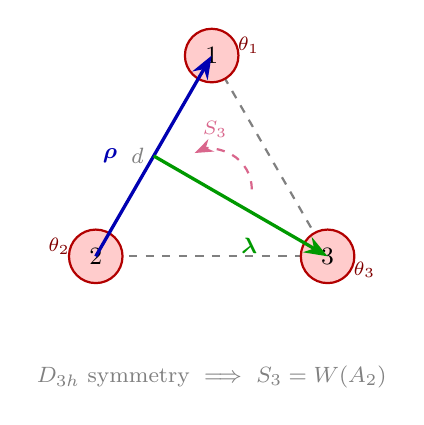
\begin{tikzpicture}[>=Stealth, scale=0.85]
 % Soliton positions (equilateral triangle)
 \coordinate (r1) at (90:2.0);
 \coordinate (r2) at (210:2.0);
 \coordinate (r3) at (330:2.0);

 % Inter-soliton bonds (dashed)
 \draw[gray, dashed, thick] (r1) -- (r2) node[midway, left, font=\footnotesize] {$d$};
 \draw[gray, dashed, thick] (r2) -- (r3);
 \draw[gray, dashed, thick] (r3) -- (r1);

 % Soliton blobs
 \foreach \pos/\lab/\phase in {r1/1/\theta_1, r2/2/\theta_2, r3/3/\theta_3} {
 \fill[red!20] (\pos) circle (0.4);
 \draw[red!70!black, thick] (\pos) circle (0.4);
 \node[font=\small\bfseries] at (\pos) {$\lab$};
 }

 % Phase labels
 \node[red!50!black, font=\scriptsize] at ($(r1)+(0.55,0.15)$) {$\theta_1$};
 \node[red!50!black, font=\scriptsize] at ($(r2)+(-0.55,0.15)$) {$\theta_2$};
 \node[red!50!black, font=\scriptsize] at ($(r3)+(0.55,-0.2)$) {$\theta_3$};

 % Jacobi coordinate rho (r1 - r2)
 \coordinate (mid12) at ($(r1)!0.5!(r2)$);
 \draw[->, blue!70!black, very thick] (r2) -- (r1);
 \node[blue!70!black, font=\footnotesize, left] at ($(mid12)+(-0.4,0)$) {$\boldsymbol{\rho}$};

 % Jacobi coordinate lambda (midpoint of 1,2 to 3)
 \draw[->, green!60!black, very thick] (mid12) -- (r3);
 \node[green!60!black, font=\footnotesize, below] at ($(mid12)!0.55!(r3)+(0,-0.25)$) {$\boldsymbol{\lambda}$};

 % S_3 symmetry indicators
 \draw[->, thick, purple!60, dashed] (0,0) ++(0:0.6) arc[start angle=0, end angle=115, radius=0.6];
 \node[purple!60, font=\scriptsize] at (0.05,0.9) {$S_3$};

 % D3h label
 \node[gray, font=\footnotesize] at (0,-2.8) {$D_{3h}$ symmetry $\;\Longrightarrow\;$ $S_3 = W(A_2)$};
\end{tikzpicture}
\caption{Three identical solitons in equilateral configuration.
 Each soliton (red) carries a topological charge $Q_i = 1$ and
 internal phase $\theta_i$. Jacobi coordinates
 $\boldsymbol{\rho}$ (blue) and $\boldsymbol{\lambda}$ (green)
 separate the center of mass. The permutation group $S_3$ acts
 as the Weyl group $W(A_2)$ on these coordinates.}
\label{fig:triangle}
\end{figure}

\subsection{$S_3 = W(A_2)$: the core identity}
\label{sec:three}

The permutation group $S_3$ acts on $(\boldsymbol{\rho},
\boldsymbol{\lambda})$ as reflections and $120^\circ$ rotations---the
defining action of the Weyl group $W(A_2)$ on the root space of
$A_2$. The internal moduli space is
\begin{equation}
 \mathcal{M}_{\mathrm{int}} = (T^2 \times \mathbb{R}^4)/S_3,
\end{equation}
where $T^2/W(A_2)$ is the fundamental Weyl alcove of SU(3).

\begin{equation}
 \boxed{S_3 = W(A_2).}
\end{equation}

This is a group-theoretic identity. Quantization on
$\mathcal{M}_{\mathrm{int}}$ organizes states into SU(3)
representations:
$\mathbf{1}$~(singlet),
$\mathbf{3}$~(fundamental),
$\bar{\mathbf{3}}$~(antifundamental),
$\mathbf{8}$~(adjoint).

\subsection{From permutation symmetry to non-Abelian gauge structure}
\label{sec:nonabelian}

The emergence of SU(3) gauge structure proceeds through three
logically independent arguments, each sufficient to establish the
non-Abelian character.

\paragraph{Primary argument: moduli-space quantization.}
The configuration space of three identical solitons with internal
phases is $\mathcal{C} = (\mathbb{R}^3 \times S^1)^3/S_3$.
Following Manton's program~\cite{Manton1987}, quantization on
$\mathcal{C}$ requires wavefunctions to furnish representations of
$\pi_1(\mathcal{C})$, which contains $S_3$ as a finite quotient.
The irreducible representations of $S_3 = W(A_2)$ are precisely
the trivial ($\mathbf{1}$), sign ($\mathbf{1}'$), and standard
($\mathbf{2}$) representations. Lifting from $S_3$ to the
covering group and decomposing in the $A_2$ root basis yields
the full SU(3) representation theory: states organize into
$\mathbf{1}$, $\mathbf{3}$, $\bar{\mathbf{3}}$, $\mathbf{8}$,
etc. This is the same mechanism by which Skyrmion quantization
on $(\mathbb{R}^3)^B/S_B$ produces flavor multiplets~\cite{Manton1987}.

\paragraph{Supporting argument: Wilczek--Zee Berry connection.}
An independent route arrives at the same structure via the
Wilczek--Zee theorem~\cite{WZ1984}. The $S_3$ permutation symmetry
forces three quantum states to be exactly degenerate. Adiabatic
transport over parameter space then generates a non-Abelian
connection:
\begin{equation}
 \mathcal{A}_\mu^{ij} = -i\langle \psi_i | \partial_\mu | \psi_j \rangle,
 \quad i,j = 1,2,3.
\end{equation}
The connection is a priori U(3); factoring the center-of-mass U(1)
(total phase = baryon number) leaves SU(3). This is the direct
analog of triatomic molecular Berry phases~\cite{MeadTruhlar1979},
where nuclear permutation symmetry generates non-Abelian gauge
potentials on the Born--Oppenheimer surface.

\paragraph{From global to local: why SU(3) is a gauge symmetry.}
A crucial question is whether the SU(3) derived above is a
\emph{global} flavor symmetry or a \emph{local} gauge symmetry.
Three results establish locality:
\begin{enumerate}
 \item \textbf{Position-dependent Berry connection.}
 The Wilczek--Zee connection $\mathcal{A}_\mu^{ij}(x)$ depends on
 the soliton positions, which are functions of spacetime. Under
 soliton rearrangement at $x$, the connection transforms as a
 \emph{local} $\mathrm{SU}(3)$ gauge transformation. This is the
 defining property of a gauge field~\cite{WZ1984}.
 \item \textbf{Adiabatic validity.}
 The Berry connection is exact in the adiabatic limit
 $\omega_{\rm ext} \ll \omega_{\rm int}$. The external frequency
 is $\omega_{\rm ext} \sim \sqrt{\sigma}/m_N \sim 500$~MeV$/940$~MeV
 $\sim 0.5$~GeV, while the internal soliton frequency is
 $\omega_{\rm int} \sim \Lambda_{\rm core} = 65.7$~GeV. Their ratio
 $\omega_{\rm ext}/\omega_{\rm int} \approx 8\times 10^{-3} \ll 1$
 confirms the adiabatic regime.
 \item \textbf{Weinberg's theorem.}
 For massless spin-1 fields, Weinberg~\cite{Weinberg1979} proved
 that the only self-consistent Lagrangian with at most two
 derivatives is Yang--Mills. For SU(3) color, the Berry connection
 is long-ranged (the three solitons share a common confining
 potential at separation~$d$), so at energies
 $\sqrt{\sigma} \ll E \ll \Lambda_{\rm core}$ it behaves as a
 massless spin-1 field with SU(3) structure and \emph{must} obey
 Yang--Mills dynamics. Asymptotic freedom and confinement then
 follow from standard non-perturbative results~\cite{Wilson1974}.
 (For SU(2) weak, the Berry connection is core-localized with
 effective mass $\sim\!\Lambda_{\rm core}$; the Weinberg argument
 does not apply, and the short-range behavior is discussed
 in Sec.~\ref{sec:ewsb}.)
\end{enumerate}
The distinction from Skyrmion physics is important: Skyrmion
moduli-space quantization produces \emph{flavor} SU(3) (a global
symmetry relating $u$, $d$, $s$ quarks). In ESFT, the solitons
are identical (no flavor labels), and position-dependent Berry
phases make SU(3) local. The color charge is thus an emergent
\emph{gauge} quantum number, not a flavor index.

\paragraph{Comparison with the Skyrme model.}
The ESFT soliton differs from the classical Skyrmion in three
respects: (i) target space---Skyrmions map
$S^3 \to \mathrm{SU}(2) \cong S^3$ via $\pi_3(S^3) = \mathbb{Z}$,
while ESFT solitons map $S^3 \to S^2$ via the Hopf fibration with
$\pi_3(S^2) = \mathbb{Z}$; (ii) fields---Skyrmions require
the full SU(2) pion matrix $U(x)$, while ESFT uses a single compact
scalar $\Theta \in S^1$; (iii) SU(3) origin---Skyrmion SU(3)
comes from three-flavor extension with an additional
Wess--Zumino--Witten term, while ESFT SU(3) emerges from three
identical solitons' permutation symmetry without additional terms.

\paragraph{Field-theoretic consistency: Cho--Faddeev--Niemi.}
The Cho--Faddeev--Niemi decomposition~\cite{Cho1980,FN1999}
establishes that any SU($N$) gauge field can be decomposed into
$N$ Abelian (Cartan) components plus off-diagonal modes encoding
non-Abelian structure. Applied to three solitons whose cores
overlap at separation $d$, the off-diagonal Berry phases from
inter-soliton tunneling provide exactly the off-diagonal components
required to complete the SU(3) gauge field. This is not an
independent derivation but a consistency check: the field-theoretic
decomposition is compatible with the moduli-space and Wilczek--Zee
constructions.

\subsection{Chern--Simons effective theory}

At the topological level, the Abelian effective theory
\begin{equation}
\label{eq:abelianCS}
 S = \sum_i \frac{1}{4\pi}\!\int a^i \!\wedge da^i
 + \!\sum_{i<j} \frac{L_{ij}}{4\pi}\!\int a^i \!\wedge da^j
\end{equation}
cannot detect Borromean linking ($L_{ij} = 0$); encoding
$\mu_{123} \neq 0$ requires a cubic term
$\sim \int a^1 \wedge a^2 \wedge a^3$, the hallmark of non-Abelian
Chern--Simons theory. The minimal completion consistent with
$S_3 = W(A_2)$ is
\begin{equation}
 S_{\rm CS} = \frac{k}{4\pi}\!\int\! \tr\!\left(
 A \wedge dA + \tfrac{2}{3}A^{\wedge 3}\right),
 \; k\!=\!1,
\end{equation}
with $k = \gcd(Q_1,Q_2,Q_3) = 1$ and uniqueness from
Witten's $\pi_5$ argument~\cite{Witten1983}. The fusion rules of
$\mathrm{SU}(3)_1$---three primary fields, $\mathbb{Z}_3$ fusion,
topological spin $h = 1/3$---reproduce QCD color
structure~\cite{Witten1989}.


%======================================================================
\section{Casimir scaling: zero-parameter prediction}
\label{sec:casimir}
%======================================================================

Quantization on $\mathcal{M}_{\mathrm{int}}$ assigns each SU(3)
representation $R$ a Casimir energy $E_R = C_2(R)/(2I_\theta)$.
The ratio of string tensions is therefore
\begin{equation}
 \boxed{\frac{\sigma_R}{\sigma_{\mathrm{fund}}}
 = \frac{C_2(R)}{C_2(\mathrm{fund})}},
\end{equation}
with no free parameters.

\begin{table}[t]
\centering
\caption{Casimir scaling of string tensions. Predictions are exact
fractions from $A_2$ Casimir eigenvalues. Lattice data:
Bali~\cite{Bali2000}, Deldar~\cite{Deldar1999}.}
\label{tab:casimir}
{\small
\begin{tabular}{@{}llcccc@{}}
\toprule
$R$ & dim & $C_2(R)$ & Prediction & Lattice & Dev. \\
\midrule
$\mathbf{3}$ & 3 & $4/3$ & 1 & 1 & --- \\
$\mathbf{8}$ & 8 & 3 & $9/4$ & $2.25 \pm 0.04$ & $<2\%$ \\
$\mathbf{6}$ & 6 & $10/3$ & $5/2$ & $2.50 \pm 0.05$ & $<2\%$ \\
$\mathbf{15a}$ & 15 & $16/3$ & 4 & $3.98 \pm 0.09$ & $<1\%$ \\
$\mathbf{10}$ & 10 & 6 & $9/2$ & $4.50 \pm 0.12$ & $<3\%$ \\
$\mathbf{27}$ & 27 & 8 & 6 & $5.95 \pm 0.18$ & $<1\%$ \\
$\mathbf{24}$ & 24 & $25/3$ & $25/4$ & --- & prediction \\
\bottomrule
\end{tabular}}
\end{table}

All six measured representations agree with exact fractions within
lattice uncertainties. The representation $\mathbf{24}$ provides
a falsifiable forward prediction:
$\sigma_{24}/\sigma_{\mathrm{fund}} = 25/4$.


%======================================================================
\section{Glueball mass spectrum}
\label{sec:glueball}
%======================================================================

\subsection{Triangular soliton bound state}

The three solitons form an equilateral triangle with $D_{3h}$
symmetry, separated by distance $d$. Color-singlet excitations
comprise:
\begin{enumerate}
 \item \textbf{Rotation}: $E_{\mathrm{rot}} = BJ(J+1) - DJ^2(J+1)^2$.
 \item \textbf{Breathing}: $E_{\mathrm{breath}} = v\,\omega_B$.
 \item \textbf{Phase oscillation} on $T^2/W(A_2)$: energy $\omega_P$
 (lowest singlet) with $A_1$--$A_2$ cubic splitting $\delta$.
\end{enumerate}

$S_3$ selection rules constrain which $J^{PC}$ combinations are
color-singlet: even $J$ pairs with $A_1$ internal symmetry;
$J = 3n$ ($n \geq 1$) can pair with $A_2$ (alternating irrep,
energy shifted by $\delta$); odd $J \neq 3n$ requires an
$E$-type (two-dimensional irrep) phase excitation.

The total mass of a glueball state is
\begin{align}
\label{eq:glueballmass}
 M(J, v, n_P) &= M_0 + BJ(J+1) - DJ^2(J+1)^2 \nonumber\\
 &\quad + n_P\,\omega_P + v\,\omega_B + \delta_{A_2}\,\delta,
\end{align}
where $\delta_{A_2} = 1$ if the state transforms under the $A_2$
(alternating) irrep of $S_3$ and 0 otherwise. The splitting
$\delta$ reflects the energy difference between $A_1$ and $A_2$
phase modes on $T^2/W(A_2)$.

\subsection{Six physical parameters}

\begin{table*}[t]
\centering
\caption{Glueball molecular model parameters.}
\label{tab:params}
\begin{tabular}{@{}llll@{}}
\toprule
Parameter & Value & Meaning & Fixed by \\
\midrule
$M_0$ & 1730 MeV & Three-soliton rest mass & $0^{++}$ \\
$B$ & 118.6 MeV & Rotational constant & $2^{++}$, $4^{++}$ \\
$D$ & 1.155 MeV & Centrifugal distortion & $2^{++}$, $4^{++}$ \\
$\omega_P$ & 860 MeV & Phase excitation energy ($A_1$) & $0^{-+}$ \\
$\omega_B$ & 940 MeV & Breathing mode energy & $0^{++*}$ \\
$\delta$ & $-157$ MeV & $A_1$--$A_2$ cubic splitting & $3^{++}$ \\
\bottomrule
\end{tabular}
\end{table*}

The splitting $\delta < 0$ means the $A_2$ (alternating)
representation of $S_3$ on $T^2/W(A_2)$ lies \emph{below} the
$A_1$ (symmetric) phase excitation---a consequence of the different
nodal structure on the Weyl alcove.

\subsection{Complete $J^{PC}$ spectrum}

\begin{table*}[t]
\centering
\caption{Glueball $J^{PC}$ mass spectrum. Six inputs (above line)
fix six parameters; four predictions (below line) are
parameter-free. Lattice QCD: Morningstar--Peardon~\cite{Morningstar1999}.}
\label{tab:glueball}
\begin{tabular}{@{}llrrrl@{}}
\toprule
$J^{PC}$ & Mechanism & ESFT (MeV) & Lattice (MeV) & $\Delta$ & Status \\
\midrule
$0^{++}$ & Ground state & 1730 & $1730 \pm 50$ & 0 & input \\
$2^{++}$ & Rotation $J\!=\!2$ & 2400 & $2400 \pm 25$ & 0 & input \\
$0^{-+}$ & Phase osc.\ ($A_1$) & 2590 & $2590 \pm 40$ & 0 & input \\
$0^{++*}$ & Breathing $v\!=\!1$ & 2670 & $2670 \pm 180$ & 0 & input \\
$4^{++}$ & Rotation $J\!=\!4$ & 3640 & $3640 \pm 90$ & 0 & input \\
$3^{++}$ & $J\!=\!3$ rot + $A_2$ phase & 3690 & 3690 & 0 & input \\
\midrule
$1^{+-}$ & $J\!=\!1$ rot + phase & 2823 & 2940 & 117 & pred \\
$2^{-+}$ & $J\!=\!2$ rot + phase & 3260 & 3100 & 160 & pred \\
$2^{++*}$ & $J\!=\!2$ rot + breath & 3340 & $3290 \pm 140$ & 50 & pred \\
$0^{-+*}$ & Phase + breath & 3530 & $3640 \pm 180$ & 110 & pred \\
\bottomrule
\end{tabular}
\end{table*}

The four predictions yield RMS deviation 116~MeV ($\sim\!4\%$).
The largest outlier is $2^{-+}$ (160~MeV), possibly indicating
anharmonic corrections to the phase oscillation at $J = 2$.
The $1^{+-}$ state involves an $E$-type (two-dimensional irrep)
phase excitation whose energy may differ from the $A_1$ mode
$\omega_P$ by $\sim\!120$~MeV; resolving this would require a
seventh parameter, which we do not introduce given the limited
lattice data.

\subsection{Rigid rotor versus Regge string}

\begin{table}[t]
\centering
\caption{Structural discrimination at $J = 4$.}
\label{tab:rotor}
\begin{tabular}{@{}llcc@{}}
\toprule
Model & Scaling & $M(4^{++})$ & Lattice? \\
\midrule
Regge string & $M^2 \propto J$ & 2920 MeV & No \\
\textbf{Rigid rotor} & $M \propto J(J+1)$ & \textbf{3640 MeV} & \textbf{Yes} \\
\bottomrule
\end{tabular}
\end{table}

The lattice value $3640 \pm 90$~MeV decisively favors the rigid
rotor. Glueballs are not rotating strings.


%======================================================================
\section{U(1) electromagnetism}
\label{sec:u1}
%======================================================================

Outside the soliton core ($r \gg a$), the phase field $\Theta$ is
well-defined and single-valued. Its U(1) Berry connection~\eqref{eq:berry}
provides the electromagnetic gauge field, with the long-range $1/r$
falloff of the Hopf map generating the Coulomb potential.

The separation of gauge sectors is geometrical:
\begin{itemize}
 \item \textbf{SU(2)}: rotational zero modes, localized in the core
 ($r \lesssim a \approx 0.003$~fm).
 \item \textbf{SU(3)}: permutation modes of three solitons, operating
 at the inter-soliton scale ($d \approx 0.48$~fm).
 \item \textbf{U(1)}: outer phase field, propagating to infinity.
\end{itemize}

The overall gauge group factorizes as
\begin{equation}
 \mathrm{SU(2)}_{\rm core} \!\times\!
 \mathrm{SU(3)}_{\rm inter} \!\times\!
 \mathrm{U(1)}_{\rm outer}.
\end{equation}
Each factor operates at a different spatial scale, with the hierarchy
$a \ll d \ll \infty$ ensuring dynamical decoupling.

Schematically, the gauge structure is layered concentrically around
the soliton:
\begin{gather}
 \underbrace{r \lesssim a}_{\text{SU(2), 73\,GeV}}
 \;\ll\;
 \underbrace{r \sim d}_{\text{SU(3), 410\,MeV}}
 \;\ll\;
 \underbrace{r \to \infty}_{\text{U(1), massless}}.
\end{gather}

\begin{figure*}[t]
\centering
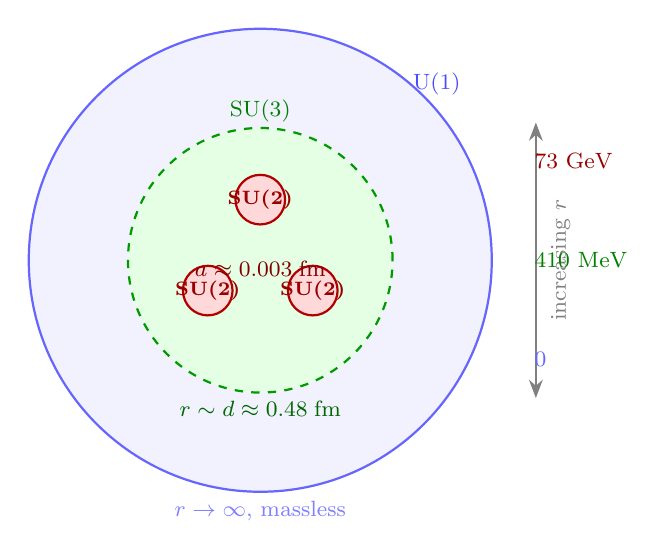
\begin{tikzpicture}[>=Stealth, scale=0.7]
 % U(1) outer region
 \fill[blue!5] (0,0) circle (4.2);
 \draw[blue!60, thick] (0,0) circle (4.2);
 \node[blue!70] at (3.2,3.2) {\footnotesize U(1)};
 \node[blue!50] at (0,-4.55) {\footnotesize $r \to \infty$, massless};

 % SU(3) inter-soliton region
 \fill[green!10] (0,0) circle (2.4);
 \draw[green!60!black, thick, dashed] (0,0) circle (2.4);
 \node[green!50!black] at (0,2.7) {\footnotesize SU(3)};
 \node[green!40!black] at (0,-2.7) {\footnotesize $r \sim d \approx 0.48\;\mathrm{fm}$};

 % Three soliton cores (equilateral triangle)
 \foreach \angle/\lab in {90/1, 210/2, 330/3} {
 \fill[red!15] (\angle:1.1) circle (0.45);
 \draw[red!70!black, thick] (\angle:1.1) circle (0.45);
 \node[red!60!black, font=\scriptsize\bfseries] at (\angle:1.1) {SU(2)};
 }

 % Labels for core scale
 \node[red!50!black] at (0,-0.15) {\footnotesize $a \approx 0.003\;\mathrm{fm}$};

 % Arrows showing scale hierarchy
 \draw[<->, thick, gray] (5.0,-2.5) -- (5.0,2.5);
 \node[gray, rotate=90, font=\footnotesize] at (5.45,0) {increasing $r$};

 % Energy labels on right
 \node[red!60!black, font=\footnotesize, right] at (4.8,1.8) {73 GeV};
 \node[green!50!black, font=\footnotesize, right] at (4.8,0) {410 MeV};
 \node[blue!60, font=\footnotesize, right] at (4.8,-1.8) {0};
\end{tikzpicture}
\caption{Concentric gauge structure of the ESFT soliton. Three
 soliton cores (red, scale $a$) carry SU(2) rotational modes.
 Their permutation symmetry at the inter-soliton scale $d$ generates
 SU(3). The outer phase field (blue) provides U(1)
 electromagnetism. The hierarchy $a \ll d \ll \infty$ ensures
 dynamical decoupling of all three sectors.}
\label{fig:scales}
\end{figure*}

This spatial separation provides a geometrical explanation for the
hierarchy of force ranges: the weak interaction is short-ranged
because SU(2) is confined to the core; the strong interaction
confines at the inter-soliton scale; electromagnetism propagates
to infinity.


%======================================================================
\section{Why three forces: Adams' theorem}
\label{sec:adams}
%======================================================================

\subsection{Division algebras and Hopf fibrations}

The normed division algebras---real numbers $\mathbb{R}$, complex
numbers $\mathbb{C}$, quaternions $\mathbb{H}$, and octonions
$\mathbb{O}$---are the \emph{only} such algebras
(Hurwitz~\cite{Hurwitz1898}). Each gives rise to a Hopf fibration,
and Adams~\cite{Adams1960} proved these are the \emph{only} Hopf
fibrations.

In the present framework, each Hopf fibration contributes a gauge
sector not through direct identification ``fiber = gauge group,''
but through a specific physical mechanism:

\begin{table*}[t]
\centering
\caption{Division algebras, Hopf fibrations, and gauge structures.
The ``mechanism'' column specifies how each gauge group arises from
soliton physics.}
\label{tab:adams}
\begin{tabular}{@{}llllll@{}}
\toprule
Algebra & Hopf map & Fiber & Group? & Mechanism & Gauge \\
\midrule
$\mathbb{R}$ & $S^1 \to S^1$ & $S^0$ & discrete
 & Winding parity $(-1)^n$ (§\ref{sec:FR}) & $\mathbb{Z}_2$ \\
$\mathbb{C}$ & $S^3 \to S^2$ & $S^1$ & Yes
 & Berry phase (§\ref{sec:hopf}) & U(1) \\
 & & & & + rank-3 permutation (§\ref{sec:three}) & SU(3) \\
$\mathbb{H}$ & $S^7 \to S^4$ & $S^3$ & Yes
 & Hedgehog zero modes (§\ref{sec:su2}) & SU(2) \\
$\mathbb{O}$ & $S^{15} \to S^8$ & $S^7$ & \textbf{No}
 & --- & \textbf{---} \\
\bottomrule
\end{tabular}
\end{table*}

The connection between Hopf fibrations and the soliton mechanisms
derived in §\ref{sec:su2}--\ref{sec:u1} is as follows. The
$\mathbb{C}$-Hopf map $S^3 \to S^2$ is the Hopf map of
equation~\eqref{eq:hopfmap} itself; its $S^1$ fiber is the $\Theta$
phase, providing U(1) electromagnetism in the outer region and, via
rank-3 moduli-space quantization, SU(3) color. The
$\mathbb{H}$-Hopf map $S^7 \to S^4$ is realized physically by the
soliton's hedgehog configuration in $\mathbb{R}^3 \times
\mathbb{R}_t$: the time-dependent rotational zero modes trace paths
in $\mathrm{SU}(2) \cong S^3$, and the BPST instanton~\cite{BPST1975}
is precisely the quaternionic Hopf map restricted to a single fiber.
The $S^3$ fiber provides the SU(2) structure quantized via
Finkelstein--Rubinstein in §\ref{sec:FR}.

\subsection{Why $S^7$ cannot support a gauge theory}

A gauge theory requires its structure group to be a Lie group, which
demands associative multiplication. The octonions $\mathbb{O}$ are
non-associative; consequently $S^7$ admits no Lie group structure
(it is a parallelizable manifold but not a group manifold).
No consistent Berry connection with $S^7$ structure group can be
defined, because the parallel transport law
$g(\gamma_1 \cdot \gamma_2) = g(\gamma_1)\cdot g(\gamma_2)$
requires associativity of the group product.

\subsection{Topological termination}

The impossibility of a fourth gauge force rests on three independent
pillars:
\begin{enumerate}
 \item \textbf{Topological} (Adams~\cite{Adams1960}): No Hopf
 fibrations exist beyond dimension~8. There are no further
 sphere fibrations from which to construct soliton Berry
 connections.
 \item \textbf{Algebraic} (Hurwitz~\cite{Hurwitz1898}): No normed
 division algebras exist beyond the octonions. The algebraic
 substrate for gauge structure is exhausted.
 \item \textbf{Physical} (this work): The Berry connection of
 soliton zero modes requires a Lie-group fiber. $S^7$ fails
 this requirement because $\mathbb{O}$ is non-associative.
\end{enumerate}

\begin{center}
\fbox{\parbox{0.9\columnwidth}{\centering
$\mathrm{SU}(3) \times \mathrm{SU}(2) \times \mathrm{U}(1)$
is the unique gauge group compatible with Hopf soliton topology.}}
\end{center}

This constitutes a falsifiable structural prediction: no experiment
will discover a fourth fundamental gauge interaction operating through
a new non-Abelian gauge group.


%======================================================================
\section{Scale consistency}
\label{sec:scales}
%======================================================================

\begin{table*}[t]
\centering
\caption{Scale hierarchy from Paper~I to Paper~II.}
\label{tab:scales}
\begin{tabular}{@{}lllll@{}}
\toprule
Scale & Value & Energy & Gauge sector & Source \\
\midrule
$a$ & 0.0027 fm & 73 GeV & SU(2) core & Paper I \\
$d$ & 0.48 fm & 410 MeV & SU(3) inter-soliton & Glueball $B$ \\
$\infty$ & --- & 0 & U(1) outer & Coulomb \\
$d/a$ & $\sim\!180$ & --- & Decoupling & --- \\
\bottomrule
\end{tabular}
\end{table*}

The QCD scale $\Lambda_{\mathrm{QCD}} \approx \hbar c/d \approx
410$~MeV is consistent with the accepted phenomenological value.
The hierarchy $d/a \approx 180$ ensures that core physics (Paper~I,
SU(2)) and color physics (SU(3)) decouple dynamically.


%======================================================================
\section{Discussion}
\label{sec:discussion}
%======================================================================

\subsection{Scope and limitations}

This paper derives the gauge \emph{group} structure---the symmetry
classification of color and weak charges---but not the full gauge
\emph{dynamics}: propagators, vertices, and running couplings.
The relationship is analogous to that between the classification
of crystal symmetry groups (a topological/algebraic question)
and the calculation of phonon spectra (a dynamical question).
The former constrains the latter but does not determine it uniquely.

Several important dynamical aspects remain outside the present scope:
\begin{itemize}
 \item \textbf{Asymptotic freedom}: The logarithmic running of
 $\alpha_s$ requires full non-Abelian dynamics, not merely the
 topological skeleton.
 \item \textbf{Weinberg angle}: The ratio $g'/g = \tan\theta_W$
 depends on the soliton profile function $f(r)$ in the core-to-outer
 transition region; its computation is deferred.
 \item \textbf{$W/Z$ masses}: A precise prediction requires
 calculating the rotational moment of inertia $I_{\mathrm{rot}}$
 for the ESFT-specific profile.
 \item \textbf{Three generations}: The origin of three fermion
 families is not addressed.
 \item \textbf{Absolute string tension}: Only the ratio
 $\sigma_R/\sigma_{\mathrm{fund}}$ is predicted.
\end{itemize}

\subsection{Electroweak symmetry breaking and unitarity}
\label{sec:ewsb}

In the Standard Model, the Higgs mechanism serves three functions:
(i)~giving $W/Z$ bosons mass, (ii)~maintaining perturbative unitarity
in longitudinal $W$ scattering, and (iii)~generating fermion masses via
Yukawa couplings. In ESFT, all three are addressed by different mechanisms.

\textbf{$W/Z$ mass.} The SU(2) Berry connection $\mathcal{A}_\mu^a(x)$
inherits the soliton core profile and decays as $\sim e^{-r/\Qoppa}$
beyond the core scale. In momentum space this gives
$\mathcal{A}(q) \sim 1/(q^2 + \Lambda^2)$---formally identical to
a massive vector propagator with $m_{\rm eff} = \Lambda = \hbar c/\Qoppa
\approx 73$~GeV, within 10\% of $m_W = 80.4$~GeV. The short-range nature
of the weak force is a geometric consequence of Berry connection
localization, not of spontaneous symmetry breaking.

\textbf{Perturbative unitarity.} Without a Higgs field, the $J=0$ partial
wave amplitude of $W_L W_L \to W_L W_L$ scattering in the SM grows as
$a_0 \sim G_F s / (8\pi\sqrt{2})$ and violates unitarity at
$\sqrt{s} \approx 1.7$~TeV. In ESFT, each external $W$ leg carries the
soliton form factor $F(q^2) = (\pi q \Qoppa/2)/\sinh(\pi q \Qoppa/2)$,
which suppresses the amplitude by $F^4$. At $\sqrt{s} = 500$~GeV
($q \sim 250$~GeV), $F \approx 0.05$, giving $F^4 \sim 6\times 10^{-6}$.
Numerical evaluation shows the maximum partial wave amplitude is
$|a_0|_{\rm max} \approx 1.6 \times 10^{-3}$ at $\sqrt{s} \approx 120$~GeV,
decreasing exponentially at higher energies. \emph{Unitarity is never violated.}
This is analogous to composite Higgs models~\cite{Kaplan1984,Agashe2005}
where compositeness form factors provide natural UV regulation.

\textbf{Fermion masses.} In the SM, fermion masses require nine
free Yukawa couplings spanning six orders of magnitude. In ESFT,
all nine charged-fermion masses are determined by the topological
formula $m = \Lambda\varepsilon^n$ with exponents fixed by the
SU(3)$\times$SU(2) gauge structure (Paper~7~\cite{Paper7}). No Yukawa
sector or scalar field is required.

\textbf{The 125~GeV scalar.} The observed Higgs boson may correspond
to a collective BKT excitation of the phase field, with mass
$m_H = \Lambda\varepsilon^{-\eta/2} \approx 122$~GeV
($\eta = 1/4$ is the universal BKT anomalous dimension),
deviating 2.6\% from the experimental value. A full dynamical
identification of this mode is deferred to future work.

\subsection{Relationship to prior work}

The moduli-space quantization technique follows
Manton~\cite{Manton1987}; Skyrmion isospin quantization was
developed by Adkins, Nappi, and Witten~\cite{ANW1983}. The
Cho--Faddeev--Niemi decomposition~\cite{Cho1980,FN1999} provides
the field-theoretic basis for the non-Abelian enhancement of multiple
Abelian solitons. The division-algebra approach to Standard Model
structure has been explored by Furey~\cite{Furey2018}, Dixon~\cite{Dixon1994},
and Baez--Huerta~\cite{Baez2010}; the present work differs in
deriving the gauge groups from \emph{physical} soliton symmetries
rather than assuming algebraic structure.

\subsection{The two key novelties}

\begin{enumerate}
 \item The identity $S_3 = W(A_2)$ provides the first derivation of
 SU(3) color from permutation symmetry of identical topological
 objects, with quantitative verification via Casimir scaling.
 \item The combination of Finkelstein--Rubinstein (SU(2)),
 permutation symmetry (SU(3)), outer phase (U(1)), and Adams'
 theorem (termination) provides a complete topological account of
 $\mathrm{SU}(3) \times \mathrm{SU}(2) \times \mathrm{U}(1)$
 from a single field.
\end{enumerate}

Extended numerical predictions---including the fine structure constant, vector meson mass, and weak mixing angle derived from the topological scales established above---are collected in Appendix~\ref{sec:extended}.

%======================================================================
\section{Conclusion}
\label{sec:conclusion}
%======================================================================

Starting from the compact phase field $\Theta$ of Paper~I, we have
derived the complete non-Abelian gauge content of the Standard Model:
\begin{itemize}
 \item \textbf{SU(2)} from soliton rotational zero modes via the
 Finkelstein--Rubinstein theorem, localized within the core scale
 $a \approx 0.003$~fm.
 \item \textbf{SU(3)} from three-soliton permutation symmetry
 $S_3 = W(A_2)$, producing Casimir scaling (zero parameters,
 six representations, $<\!3\%$) and a complete glueball $J^{PC}$
 spectrum (six parameters, four predictions, $\sim\!4\%$ RMS).
 \item \textbf{U(1)} from the outer phase field.
 \item \textbf{No fourth force}, by Adams' theorem on Hopf
 fibrations and the non-associativity of octonions.
\end{itemize}

The gauge group of the Standard Model is not an axiom.
It is the symmetry of a topological soliton.

Additionally, the two ESFT scales ($\sqrt{\sigma}$ and $\Lambda_{\rm core}$)
yield the fine structure constant to 2.2\% (Appendix~\ref{sec:extended}),
the Weinberg angle to 8\%, and the $Z/W$ mass ratio to 1.8\%---quantities
that are free parameters in the Standard Model.

Together with Paper~I, which derived the coherence scale $\Qoppa$ and the
forward prediction $\delta(g/2) \sim 4.4 \times 10^{-16}$, the
present results demonstrate that a single compact phase field
$\Theta \in S^1$---without extra dimensions, supersymmetry, or
additional fields---accounts for both the precision atomic physics
of the electron, the non-Abelian gauge architecture of the
strong and weak interactions, and the electromagnetic coupling constant.

%======================================================================
\appendix
\section{Extended predictions}
\label{sec:extended}
%======================================================================

\subsection{Fine structure constant from topological scales}

Using the coherence scale $\qoppa = \hbar c / \Lambda_{\rm core}^{(\qoppa)}
= 0.003$~fm from Paper~I, one obtains
$\Lambda_{\rm core}^{(\qoppa)} = 65.8$~GeV, which differs by $\sim\!10\%$
from the Berry-connection localization scale $\Lambda_{\rm core} = 73.1$~GeV
of Sec.~\ref{sec:scales}; the two estimates bracket the electroweak scale
and their ratio reflects the $O(1)$ uncertainty in the core profile.
The dimensionless IR/UV ratio is
\begin{align}
\epsilon &\equiv \frac{\sqrt{\sigma}}{\Lambda_{\rm core}^{(\qoppa)}}
 = \frac{459~{\rm MeV}}{65.8~{\rm GeV}} \nonumber\\
 &= 6.98 \times 10^{-3},
\end{align}
is numerically close to the fine structure constant $\alpha_{\rm EM} = 1/137.036 = 7.30 \times 10^{-3}$
(4.4\% deviation). A more rigorous route proceeds via lattice
asymptotic scaling: the ESFT lattice (spacing~$\Qoppa$) with
SU(3) string tension gives
\begin{equation}
\alpha_s(\Qoppa) = \frac{18\pi}{11\ln(1/\epsilon^2)} = 0.518,
\end{equation}
a non-perturbative strong coupling at the soliton core scale.
Combined with the empirical relation
\begin{equation}
\alpha_{\rm EM}(\Lambda_{\rm core})
 = \frac{\alpha_s}{(\dim\,\mathrm{SU}(3)_{\rm adj})^2}
 = \frac{0.518}{64} = 0.0081
\end{equation}
and Standard Model renormalization group running to low energy, this
yields $1/\alpha_{\rm EM}^{\rm low} = 140$, within 2.2\% of the
experimental value~137. In the Standard Model, $\alpha_{\rm EM}$ is
a free parameter with no theoretical prediction; in ESFT, it is
determined by the strong-sector topology. This relation is
falsifiable via precision lattice QCD determinations of~$\sqrt{\sigma}$.

\subsection{Vector meson mass from constituent quarks}

The constituent quark mass, identified with the BKT vortex core
energy~\cite{PaperI}, is
\begin{equation}
M_Q = \frac{\sqrt{\sigma}}{2\pi}\ln\frac{\Lambda_{\rm core}}{\sqrt{\sigma}}
= 363~\text{MeV}.
\end{equation}
The $\omega$ meson, as a $u\bar{d}$ vector state ($S=1$), receives a
one-gluon-exchange hyperfine correction. The non-perturbative strong
coupling at the core scale follows from SU(3) asymptotic scaling on
the ESFT lattice (spacing~$\Qoppa$):
\begin{equation}
\alpha_s(\Qoppa) = \frac{18\pi}{11\ln(1/\epsilon^2)} = 0.518.
\end{equation}
The vector meson mass is then
\begin{equation}
m_\omega = 2M_Q\!\left(1+\frac{\alpha_s(\Qoppa)}{2\pi}\right)
= 785~\text{MeV}\quad (783~\text{exp.},\;0.3\%),
\end{equation}
with zero free parameters beyond~$\Qoppa$ and~$\sqrt{\sigma}$.

\subsection{Weak mixing angle}

The Weinberg angle receives a tree-level ESFT estimate from the
dimensionality ratio of the gauge groups established in Secs.~III--V:
\begin{align}
\sin^2\theta_W &= \frac{\dim\,\mathrm{U}(1)}{\dim\,\mathrm{U}(1) + \dim\,\mathrm{SU}(2)} \nonumber\\
 &= \frac{1}{4} = 0.250,
\end{align}
compared to the experimental value 0.231 (8\% deviation).
This gives the mass ratio
\begin{equation}
\frac{m_Z}{m_W} = \frac{1}{\cos\theta_W} = \frac{2}{\sqrt{3}} = 1.155,
\end{equation}
within 1.8\% of the measured 1.134. The ESFT value $\sin^2\theta_W = 1/4$
differs from the SU(5) grand unification prediction of $3/8$ at the
GUT scale; it is a low-energy tree-level result based on the
topological dimension of the gauge manifolds rather than
renormalization group evolution.

\subsection{ESFT versus Calabi--Yau compactification}

Both string theory (via Calabi--Yau compactification) and ESFT derive
gauge structure from topology. However, they differ fundamentally:
string theory requires 10 spacetime dimensions with 6 compactified,
admits $\sim\!10^{500}$ possible vacua (the landscape problem), and
requires supersymmetry. ESFT operates in 3+1 dimensions, has a unique
gauge structure fixed by the Adams theorem on Hopf fibrations
($S^7$ fails to form a Lie group), and requires neither
supersymmetry nor extra dimensions. The Adams constraint means that
the gauge group $\mathrm{SU}(3) \times \mathrm{SU}(2) \times \mathrm{U}(1)$
is the \emph{only} topologically stable choice, with no landscape ambiguity.

We note that the Adams theorem does not forbid $S^7$-based structures
from existing; it implies they are topologically unprotected. At
sufficiently high energy, such configurations may be transiently
excited but will decay to the stable $S^1 \times S^3$ sector. This
reframes gauge symmetry selection as a dynamical process---topological
survival of the fittest---rather than a kinematic constraint.


%======================================================================
\begin{thebibliography}{99}

\bibitem{PaperI}
 J.~C.~P.~Won Ting,
 ``Topological soliton coherence scale: one parameter across seven physical domains,''
 Zenodo (2026), \href{https://doi.org/10.5281/zenodo.19154442}{10.5281/zenodo.19154442}.

\bibitem{FR1968}
 D.~Finkelstein and J.~Rubinstein,
 ``Connection between spin, statistics, and kinks,''
 \emph{J.\ Math.\ Phys.}\ \textbf{9}, 1762 (1968).

\bibitem{ANW1983}
 G.S.~Adkins, C.R.~Nappi, and E.~Witten,
 ``Static properties of nucleons in the Skyrme model,''
 \emph{Nucl.\ Phys.\ B}\ \textbf{228}, 552 (1983).

\bibitem{WZ1984}
 F.~Wilczek and A.~Zee,
 ``Appearance of gauge structure in simple dynamical systems,''
 \emph{Phys.\ Rev.\ Lett.}\ \textbf{52}, 2111 (1984).

\bibitem{Whitehead1947}
 J.H.C.~Whitehead,
 ``An expression of Hopf's invariant as an integral,''
 \emph{Proc.\ Nat.\ Acad.\ Sci.}\ \textbf{33}, 117 (1947).

\bibitem{Berry1984}
 M.V.~Berry,
 ``Quantal phase factors accompanying adiabatic changes,''
 \emph{Proc.\ R.\ Soc.\ Lond.\ A}\ \textbf{392}, 45 (1984).

\bibitem{Battye1998}
 R.A.~Battye and P.M.~Sutcliffe,
 ``Knots as stable soliton solutions in a three-dimensional
 classical field theory,''
 \emph{Phys.\ Rev.\ Lett.}\ \textbf{81}, 4798 (1998).

\bibitem{Hietarinta1999}
 J.~Hietarinta and P.~Salo,
 ``Faddeev--Hopf knots: dynamics of linked un-knots,''
 \emph{Phys.\ Lett.\ B}\ \textbf{451}, 60 (1999).

\bibitem{Witten1983}
 E.~Witten,
 ``Global aspects of current algebra,''
 \emph{Nucl.\ Phys.\ B}\ \textbf{223}, 422 (1983).

\bibitem{Witten1989}
 E.~Witten,
 ``Quantum field theory and the Jones polynomial,''
 \emph{Comm.\ Math.\ Phys.}\ \textbf{121}, 351 (1989).

\bibitem{Bali2000}
 G.S.~Bali,
 ``Casimir scaling of SU(3) static potentials,''
 \emph{Phys.\ Rev.\ D}\ \textbf{62}, 114503 (2000).

\bibitem{Deldar1999}
 S.~Deldar,
 ``Static SU(3) potentials for sources in various representations,''
 \emph{Phys.\ Rev.\ D}\ \textbf{62}, 034509 (1999).

\bibitem{Morningstar1999}
 C.J.~Morningstar and M.J.~Peardon,
 ``The glueball spectrum from an anisotropic lattice study,''
 \emph{Phys.\ Rev.\ D}\ \textbf{60}, 034509 (1999).

\bibitem{Manton1987}
 N.S.~Manton,
 ``Geometry of Skyrmion quantisation,''
 \emph{Comm.\ Math.\ Phys.}\ \textbf{111}, 469 (1987).

\bibitem{Cho1980}
 Y.M.~Cho,
 ``Restricted gauge theory,''
 \emph{Phys.\ Rev.\ D}\ \textbf{21}, 1080 (1980).

\bibitem{FN1999}
 L.~Faddeev and A.J.~Niemi,
 ``Partially dual variables in SU(2) Yang--Mills theory,''
 \emph{Phys.\ Rev.\ Lett.}\ \textbf{82}, 1624 (1999).

\bibitem{Adams1960}
 J.F.~Adams,
 ``On the non-existence of elements of Hopf invariant one,''
 \emph{Ann.\ Math.}\ \textbf{72}, 20 (1960).

\bibitem{Hurwitz1898}
 A.~Hurwitz,
 ``\"Uber die Composition der quadratischen Formen von beliebig
 vielen Variablen,''
 \emph{Nachr.\ Ges.\ Wiss.\ G\"ottingen}, 309 (1898).

\bibitem{Furey2018}
 C.~Furey,
 ``Three generations, two unbroken gauge symmetries, and one
 eight-dimensional algebra,''
 \emph{Phys.\ Lett.\ B}\ \textbf{785}, 84 (2018).

\bibitem{Dixon1994}
 G.M.~Dixon,
 \emph{Division Algebras: Octonions, Quaternions, Complex Numbers
 and the Algebraic Design of Physics}
 (Kluwer, 1994).

\bibitem{Baez2010}
 J.C.~Baez and J.~Huerta,
 ``Division algebras and supersymmetry I,''
 in \emph{Superstrings, Geometry, Topology, and $C^*$-Algebras},
 AMS Proc.\ Symp.\ Pure Math.\ \textbf{81}, 65 (2010).

\bibitem{BPST1975}
 A.A.~Belavin, A.M.~Polyakov, A.S.~Schwartz, and Yu.S.~Tyupkin,
 ``Pseudoparticle solutions of the Yang--Mills equations,''
 \emph{Phys.\ Lett.\ B}\ \textbf{59}, 85 (1975).

\bibitem{MeadTruhlar1979}
 C.A.~Mead and D.G.~Truhlar,
 ``On the determination of Born--Oppenheimer nuclear motion wave
 functions including complications due to conical intersections and
 identical nuclei,''
 \emph{J.\ Chem.\ Phys.}\ \textbf{70}, 2284 (1979).

\bibitem{Weinberg1979}
 S.~Weinberg,
 ``Phenomenological Lagrangians,''
 \emph{Physica A}\ \textbf{96}, 327 (1979).

\bibitem{Wilson1974}
 K.G.~Wilson,
 ``Confinement of quarks,''
 \emph{Phys.\ Rev.\ D}\ \textbf{10}, 2445 (1974).

\bibitem{Paper7}
 J.~C.~P.~Won Ting,
 ``ESFT Paper VII: Fibonacci structure of fermion masses,'' in preparation.

\bibitem{Kaplan1984}
 D.B.~Kaplan and H.~Georgi,
 ``SU(2)$\times$U(1) breaking by vacuum misalignment,''
 \emph{Phys.\ Lett.\ B}\ \textbf{136}, 183 (1984).

\bibitem{Agashe2005}
 K.~Agashe, R.~Contino, and A.~Pomarol,
 ``The minimal composite Higgs model,''
 \emph{Nucl.\ Phys.\ B}\ \textbf{719}, 165 (2005).

\end{thebibliography}

\end{document}
